\chapter{Architectural design}
\begin{redbar}
La \textbf{progettazione architetturale} si occupa di comprendere come dovrebbe essere organizzato un sistema software e di progettare la struttura complessiva del sistema. Essa rappresenta il collegamento fondamentale tra progettazione e ingegneria dei requisiti, poiché identifica i principali componenti strutturali di un sistema e le relazioni tra loro. L'output del processo di progettazione architetturale è un modello architetturale che descrive come il sistema è organizzato come un insieme di componenti che comunicano tra loro.
\end{redbar}

Nei processi agili, è generalmente accettato che una fase iniziale del processo di sviluppo agile si concentri sulla progettazione dell'architettura del sistema nel suo insieme. Rifattorizzare i componenti in risposta ai cambiamenti è solitamente piuttosto semplice; tuttavia, rifattorizzare l'architettura del sistema è costoso, poiché potrebbe essere necessario modificare la maggior parte dei componenti del sistema per adattarli ai cambiamenti architetturali.

Per aiutarti a capire cosa si intende per architettura di sistema, osserva la Figura \ref{fig:architecture-packing-robot}. Questo diagramma mostra un modello astratto dell'architettura di un sistema robotico di imballaggio. Questo sistema robotico è in grado di imballare diversi tipi di oggetti, usando un componente di visione per selezionare gli oggetti su un nastro trasportatore, identificarne il tipo e scegliere il tipo di imballaggio corretto. Il sistema poi trasferisce gli oggetti dal nastro trasportatore alla zona di imballaggio e deposita gli oggetti confezionati su un altro nastro trasportatore. Il modello architetturale mostra questi componenti e i collegamenti tra di loro.

\begin{figure}[ht]
    \centering
    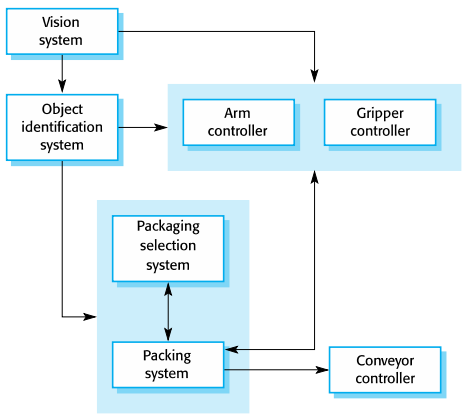
\includegraphics[width=0.45\linewidth]{images/architecture-packing-robot.PNG}
    \caption{L'architettura di un sistema di controllo del robot di imballaggio}
    \label{fig:architecture-packing-robot}
\end{figure}

Si possono progettare le architetture software a due livelli di astrazione, denominati "architettura in piccolo" e "architettura in grande":
\begin{enumerate}
    \item Architettura in piccolo riguarda l'architettura di singoli programmi, concentrandosi su come ciascun programma viene scomposto in componenti.
    \item Architettura in grande si occupa dell'architettura di sistemi complessi, come i sistemi aziendali, che includono altri sistemi, programmi e componenti di programma. Questi sistemi possono essere distribuiti su diversi computer, gestiti da aziende differenti.
\end{enumerate}
Progettare e documentare esplicitamente l'architettura software ha tre vantaggi principali:
\begin{enumerate}
    \item \textit{Comunicazione con gli stakeholder:} l'architettura è una rappresentazione ad alto livello del sistema che può essere usata come punto di discussione tra diversi stakeholder.
    \item \textit{Analisi del sistema:} le decisioni di progettazione architetturale hanno un profondo effetto sul fatto che il sistema possa soddisfare requisiti critici come prestazioni, affidabilità e manutenibilità.
    \item \textit{Riutilizzo su larga scala:} l'architettura del sistema è spesso la stessa per sistemi con requisiti simili e può quindi supportare il riutilizzo software su larga scala.
\end{enumerate}
Le architetture di sistema sono spesso modellate informalmente utilizzando semplici diagrammi a blocchi, come nella Figura \ref{fig:architecture-packing-robot}. Ogni riquadro rappresenta un componente; i riquadri interni indicano che il componente è stato scomposto in sottocomponenti. Le frecce indicano che dati o segnali di controllo vengono trasmessi da un componente all'altro nella direzione delle frecce. Tuttavia, non si considerano i diagrammi a blocchi come buone rappresentazioni architetturali poiché questi diagrammi non mostrano il tipo di relazioni tra i componenti del sistema né le proprietà visibili esternamente dei componenti.

I diagrammi a blocchi supportano efficacemente la comunicazione tra i partecipanti alla progettazione software, facilitando la comprensione da parte di esperti di dominio, ingegneri e manager. Tuttavia, per una documentazione dettagliata dell'architettura, è preferibile usare notazioni più rigorose, come i linguaggi di descrizione architetturale, che riducono la possibilità di incomprensioni.

\begin{enumerate}
    \item Come mezzo per facilitare la discussione sulla progettazione del sistema: una visione architetturale ad alto livello è utile per comunicare con gli stakeholder e per la pianificazione del progetto, poiché non è sovraccarica di dettagli.
    \item Come documentazione di un'architettura progettata: l'obiettivo qui è produrre un modello di sistema completo che mostri i diversi componenti del sistema, le loro interfacce e connessioni.
\end{enumerate}

\section{Decisioni di architectural design}
La progettazione architetturale è un processo creativo in cui si organizza un sistema in modo che soddisfi i requisiti funzionali e non funzionali. Non esiste una formula predefinita per la progettazione architetturale: essa dipende dal tipo di sistema in fase di sviluppo, dal background e dall'esperienza dell'architetto e dai requisiti specifici del sistema. Pertanto, è più utile considerare la progettazione architetturale come una serie di decisioni piuttosto che come una sequenza di attività.

Durante il processo di progettazione architetturale, gli architetti devono prendere decisioni strutturali che influenzano in modo profondo sia il sistema che il suo sviluppo. Sulla base della loro esperienza e conoscenza, essi devono considerare le domande fondamentali riportate nella Figura \ref{fig:architectural-design-decisions}.

\begin{figure}[ht]
    \centering
    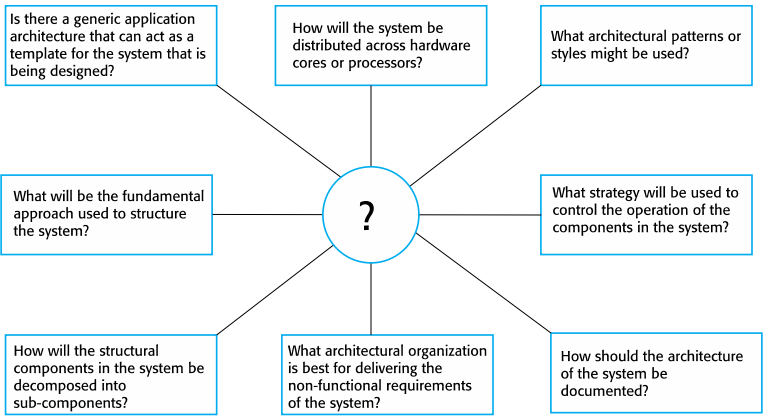
\includegraphics[width=0.7\linewidth]{images/architectural-design-decisions.PNG}
    \caption{Decisioni di architectural design}
    \label{fig:architectural-design-decisions}
\end{figure}

Sebbene ogni sistema software sia unico, i sistemi appartenenti allo stesso dominio applicativo spesso condividono architetture simili, che riflettono i concetti fondamentali del dominio. Ad esempio, le linee di prodotto applicative sono costruite attorno a un’architettura centrale con varianti per soddisfare requisiti specifici dei clienti. Nella progettazione dell'architettura di un sistema, è quindi necessario determinare cosa il sistema e le sue categorie applicative più ampie abbiano in comune e quanto delle conoscenze architetturali disponibili sia riutilizzabile.

Poiché esiste una stretta relazione tra le caratteristiche non funzionali di un sistema e la sua architettura software, la scelta dello stile e della struttura architetturale dovrebbe dipendere dai requisiti non funzionali del sistema:
\begin{enumerate}
    \item \textit{Prestazioni:} l'architettura dovrebbe essere progettata per localizzare le operazioni critiche in un numero limitato di componenti. Questo potrebbe comportare l’uso di pochi componenti relativamente grandi anziché di componenti di dimensioni più ridotte.
    \item \textit{Sicurezza:} è preferibile utilizzare una struttura stratificata, con le risorse più critiche protette negli strati più interni e sottoposte a una rigorosa validazione di sicurezza.
    \item \textit{Sicurezza operativa:} l'architettura dovrebbe essere progettata in modo che le operazioni critiche siano concentrate in un solo componente o in pochi componenti.
    \item \textit{Disponibilità:} l'architettura dovrebbe includere componenti ridondanti per consentire la sostituzione e l'aggiornamento dei componenti senza interrompere il sistema.
    \item \textit{Manutenibilità:} l'architettura dovrebbe utilizzare componenti a grana fine e autonomi che possano essere modificati facilmente.
\end{enumerate}

\section{Architectural views}
In questa sezione, affronterò due questioni rilevanti per entrambi questi scopi:
\begin{enumerate}
    \item Quali viste o prospettive sono utili nella progettazione e nella documentazione dell’architettura di un sistema?
    \item Quali notazioni dovrebbero essere utilizzate per descrivere i modelli architetturali?
\end{enumerate}
È impossibile rappresentare tutte le informazioni rilevanti sull’architettura di un sistema in un unico diagramma, poiché un modello grafico può mostrare solo una vista o una prospettiva del sistema. Potrebbe, ad esempio, mostrare come il sistema è suddiviso in moduli, come i processi interagiscono a runtime, o come i componenti del sistema sono distribuiti in rete. Poiché tutte queste prospettive sono utili in diversi momenti sia per la progettazione che per la documentazione, di solito è necessario presentare più viste dell'architettura software.

Esistono opinioni diverse su quali viste siano necessarie. Krutchen, nel suo famoso modello di architettura software "4+1 view", suggerisce quattro viste architetturali fondamentali, che possono essere collegate attraverso casi d'uso o scenari comuni (Figura \ref{fig:architectural-views}). Egli propone le seguenti viste:

\begin{figure}[ht]
    \centering
    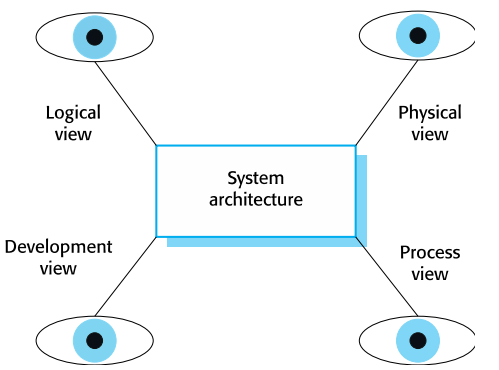
\includegraphics[width=0.4\linewidth]{images/architectural-views.PNG}
    \caption{Architectural views}
    \label{fig:architectural-views}
\end{figure}

\begin{enumerate}
    \item Una vista logica, che mostra le astrazioni chiave del sistema come oggetti o classi di oggetti.
    \item Una vista di processo, che mostra come, durante l’esecuzione, il sistema è composto da processi interagenti.
    \item Una vista di sviluppo, che mostra come il software è scomposto per lo sviluppo; in altre parole, mostra la suddivisione del software in componenti implementati da singoli sviluppatori o team di sviluppo.
    \item Una vista fisica, che mostra l’hardware del sistema e come i componenti software sono distribuiti sui processori del sistema.
    \item Casi d'uso o scenari correlati (+1).
\end{enumerate}
Ci sono opinioni divergenti riguardo l'uso dell'UML per descrivere e documentare le architetture software. L'UML è stato progettato per descrivere sistemi orientati agli oggetti e, nella fase di progettazione architetturale, spesso si desidera descrivere sistemi a un livello di astrazione superiore. Le classi di oggetti sono troppo vicine all'implementazione per essere utili nella descrizione architetturale. Non trovo l'UML particolarmente utile durante il processo di progettazione e preferisco notazioni informali, più veloci da scrivere e facilmente disegnabili su una lavagna. L'UML è più utile quando si documenta un'architettura in dettaglio o si utilizza lo sviluppo basato su modelli.

Diversi ricercatori hanno proposto l'uso di linguaggi descrittivi dell’architettura più specializzati (ADL) per descrivere le architetture dei sistemi. Tuttavia, essendo linguaggi specialistici, gli ADL sono difficili da comprendere e utilizzare per gli specialisti di dominio e applicazioni.

\section{Architectural patterns}
L'idea dei pattern come strumento per presentare, condividere e riutilizzare conoscenze sui sistemi software è stata adottata in vari ambiti dell'ingegneria del software. Si può pensare a un pattern architetturale come a una descrizione stilizzata e astratta delle buone pratiche, sperimentata e testata in diversi sistemi e ambienti. Un pattern architetturale dovrebbe quindi descrivere un'organizzazione del sistema che è risultata efficace in sistemi precedenti. Dovrebbe includere informazioni su quando è appropriato o meno utilizzare quel pattern, oltre a dettagli sui punti di forza e di debolezza del pattern.

\begin{table}[ht]
\centering
\rowcolors{2}{lightblue}{lightgray}
\begin{tabular}{|p{3cm}|p{11.5cm}|}
\hline
\rowcolor{headerblue}
\textbf{\textcolor{white}{Nome}} & \textbf{\textcolor{white}{MVC (Model-View-Controller)}} \\\hline
Descrizione & Separa la presentazione e l'interazione dai dati del sistema. Il sistema è strutturato in tre componenti logiche che interagiscono tra loro. Il componente Modello gestisce i dati del sistema e le operazioni associate su tali dati. Il componente Vista definisce e gestisce come i dati vengono presentati all'utente. Il componente Controller gestisce l'interazione dell'utente (ad esempio, pressioni dei tasti, clic del mouse, ecc.) e passa queste interazioni alla Vista e al Modello. Vedi Figura \ref{fig:graph-mvc}.\\\hline
Esempio & La Figura \ref{fig:graph-mvc} mostra l'architettura di un sistema di applicazione web organizzato utilizzando il pattern MVC.\\\hline
Quando utilizzato & Utilizzato quando ci sono modi diversi per visualizzare e interagire con i dati. Utilizzato anche quando i requisiti futuri per l'interazione e la presentazione dei dati sono sconosciuti.\\\hline
Vantaggi & Permette ai dati di cambiare indipendentemente dalla loro rappresentazione e viceversa. Supporta la presentazione degli stessi dati in modi diversi, con le modifiche apportate in una rappresentazione visualizzate in tutte.\\\hline
Svantaggi & Può comportare codice aggiuntivo e una complessità del codice maggiore quando il modello dei dati e le interazioni sono semplici.
\\\hline
\end{tabular}
\caption{La struttura di un documento di requisiti}
\label{tab:mvc-pattern}
\end{table}

La Tabella \ref{tab:mvc-pattern} descrive il famoso pattern Model-View-Controller. Questo pattern è alla base della gestione dell'interazione in molti sistemi web-based ed è supportato da numerosi framework di linguaggi di programmazione.

I modelli grafici dell'architettura associata al pattern MVC sono mostrati nella Figura \ref{fig:graph-mvc}. Questi presentano l'architettura da diverse prospettive: una vista concettuale e un'architettura del sistema a runtime quando questo pattern viene utilizzato per la gestione dell'interazione in un sistema web-based.

\begin{figure}[ht]
    \centering
    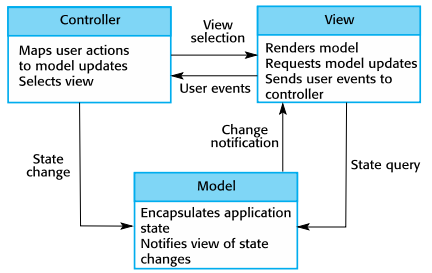
\includegraphics[width=0.45\linewidth]{images/organization-mvc.PNG}
    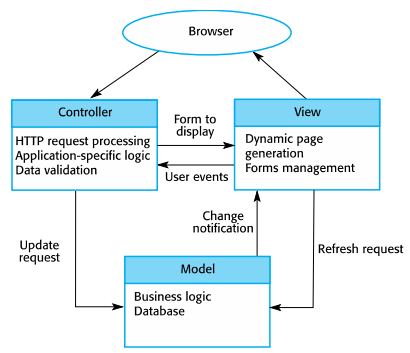
\includegraphics[width=0.45\linewidth]{images/web-app-mvc.PNG}
    \caption{Modelli grafici del Model-View-Controller}
    \label{fig:graph-mvc}
\end{figure}

Vengono presentati alcuni esempi selezionati di pattern ampiamente utilizzati e che riflettono buoni principi di progettazione architetturale.

\subsection{Layered architecture}
Il pattern dell’architettura a Livelli è un altro modo per ottenere separazione e indipendenza. Questo pattern è mostrato nella Tabella \ref{tab:layer-pattern}. Qui, la funzionalità del sistema è organizzata in livelli separati, e ogni livello si basa solo sui servizi e le funzionalità offerti dal livello immediatamente sottostante.

\begin{table}[ht]
\centering
\rowcolors{2}{lightblue}{lightgray}
\begin{tabular}{|p{3cm}|p{11.5cm}|}
\hline
\rowcolor{headerblue}
\textbf{\textcolor{white}{Nome}} & \textbf{\textcolor{white}{Architettura a livelli}} \\\hline
Descrizione & Organizza il sistema in livelli con funzionalità correlate associate a ciascun livello. Un livello fornisce servizi al livello sopra di esso, quindi i livelli più bassi rappresentano servizi di base probabilmente usati in tutto il sistema. Vedi Figura \ref{fig:layered-architecture}.\\\hline
Esempio & Un modello a livelli di un sistema per la condivisione di documenti con copyright conservati in biblioteche diverse, come mostrato in Figura \ref{fig:layered-architecture}.\\\hline
Quando utilizzato & Utilizzato quando si costruiscono nuove funzionalità su sistemi esistenti; quando lo sviluppo è suddiviso tra più team, ciascuno responsabile di un livello di funzionalità; quando è richiesto un sistema con sicurezza multi-livello.\\\hline
Vantaggi & Consente la sostituzione di interi livelli purché l'interfaccia sia mantenuta. Possono essere forniti servizi ridondanti (es. autenticazione) in ogni livello per aumentare l'affidabilità del sistema.\\\hline
Svantaggi & In pratica, è spesso difficile fornire una separazione netta tra i livelli e un livello alto può dover interagire direttamente con i livelli inferiori anziché tramite il livello immediatamente sottostante. Le prestazioni possono essere un problema a causa dei multipli livelli di interpretazione di una richiesta di servizio, mentre essa viene elaborata in ciascun livello.
\\\hline
\end{tabular}
\caption{Il modello di architettura a strati}
\label{tab:layer-pattern}
\end{table}

Questo approccio a livelli supporta lo sviluppo incrementale dei sistemi. Durante lo sviluppo di un livello, alcuni dei servizi forniti possono essere resi disponibili agli utenti. Inoltre, quando le interfacce dei livelli cambiano o si aggiungono nuove funzionalità a un livello, solo il livello adiacente ne risente. Poiché i sistemi a livelli localizzano le dipendenze dalla macchina, diventa più facile fornire implementazioni multi-piattaforma di un sistema applicativo.

\begin{figure}[ht]
    \centering
    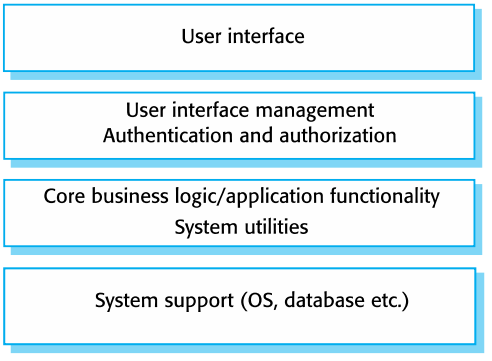
\includegraphics[width=0.40\linewidth]{images/layered-architecture.PNG}
    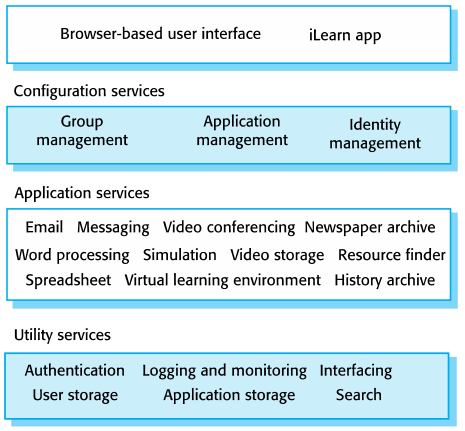
\includegraphics[width=0.45\linewidth]{images/architecture-ilean-system.PNG}
    \caption{Modelli grafici del layered architecture}
    \label{fig:layered-architecture}
\end{figure}

La Figura \ref{fig:layered-architecture} è un esempio di un’architettura a livelli con quattro livelli. Il livello più basso include il software di supporto al sistema, tipicamente supporto per database e sistema operativo. Il livello successivo è quello applicativo, che comprende i componenti relativi alla funzionalità dell’applicazione e componenti di utilità utilizzati da altri componenti applicativi.

Il terzo livello riguarda la gestione dell’interfaccia utente e fornisce autenticazione e autorizzazione per l'utente, mentre il livello superiore offre le funzionalità dell’interfaccia utente. Ovviamente, il numero di livelli è arbitrario.

\subsection{Repository architecture}
Il pattern Repository (Tabella \ref{tab:repository-architecture}), descrive come un insieme di componenti interagenti possa condividere i dati. La maggior parte dei sistemi che gestiscono grandi quantità di dati è organizzata attorno a un database condiviso o a un repository. Questo modello è quindi adatto per applicazioni in cui i dati sono generati da un componente e utilizzati da un altro.

\begin{table}[ht]
\centering
\rowcolors{2}{lightblue}{lightgray}
\begin{tabular}{|p{3cm}|p{11.5cm}|}
\hline
\rowcolor{headerblue}
\textbf{\textcolor{white}{Nome}} & \textbf{\textcolor{white}{Repository}} \\\hline
Descrizione & Tutti i dati in un sistema sono gestiti in un repository centrale accessibile a tutti i componenti del sistema. I componenti non interagiscono direttamente, ma solo attraverso il repository.\\\hline
Esempio & La Figura \ref{fig:repository-architecture} mostra un esempio di IDE in cui i componenti utilizzano un repository di informazioni di progettazione del sistema. Ogni strumento software genera informazioni che sono poi disponibili per altri strumenti.\\\hline
Quando utilizzarlo & Dovresti usare questo pattern quando hai un sistema in cui vengono generati grandi volumi di informazioni che devono essere memorizzate a lungo termine. È utile anche in sistemi guidati dai dati, dove l'inserimento di dati nel repository attiva un'azione o uno strumento.\\\hline
Vantaggi & I componenti possono essere indipendenti non hanno bisogno di conoscere l'esistenza di altri componenti. Le modifiche apportate da un componente possono essere propagate a tutti gli altri. Tutti i dati possono essere gestiti in modo coerente (ad esempio, i backup vengono eseguiti nello stesso momento), poiché sono tutti in un unico luogo.\\\hline
Svantaggi & Il repository è un singolo punto di guasto, quindi eventuali problemi nel repository influenzano l'intero sistema. Possono esserci inefficienze nell'organizzare tutte le comunicazioni attraverso il repository. Distribuire il repository su più computer potrebbe risultare difficile.
\\\hline
\end{tabular}
\caption{Il modello repository}
\label{tab:repository-architecture}
\end{table}

La Figura \ref{fig:repository-architecture} illustra una situazione in cui potrebbe essere utilizzato un repository. Questo diagramma mostra un ambiente di sviluppo integrato (IDE) che include diversi strumenti per supportare lo sviluppo basato su modelli.

\begin{figure}[ht]
    \centering
    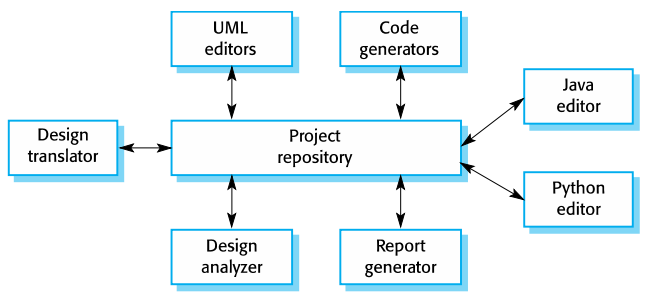
\includegraphics[width=0.55\linewidth]{images/repository-architecture-ide.PNG}
    \caption{Un'architettura di repository per un IDE}
    \label{fig:repository-architecture}
\end{figure}

Organizzare strumenti attorno a un repository è un modo efficiente per condividere grandi quantità di dati. Non è necessario trasmettere i dati esplicitamente da un componente all'altro. Tuttavia, i componenti devono operare su un modello di dati del repository concordato.

\subsection{Client–server architecture}
Il pattern Client-Server (Tabella \ref{tab:client-server-pattern}), illustra un'organizzazione comunemente utilizzata in fase di esecuzione per sistemi distribuiti. Un sistema che segue il pattern Client-Server è organizzato come un insieme di servizi e server associati, e di client che accedono e utilizzano i servizi. I principali componenti di questo modello sono:
\begin{enumerate}
    \item Un insieme di server che offrono servizi ad altri componenti. Esempi di server includono server di stampa, server di file e un server di compilazione.
    \item Un insieme di client che richiedono i servizi offerti dai server.
    \item Una rete che permette ai client di accedere a questi servizi.
\end{enumerate}

\begin{table}[ht]
\centering
\rowcolors{2}{lightblue}{lightgray}
\begin{tabular}{|p{3cm}|p{11.5cm}|}
\hline
\rowcolor{headerblue}
\textbf{\textcolor{white}{Nome}} & \textbf{\textcolor{white}{Client-server}} \\\hline
Descrizione & In un'architettura client-server, la funzionalità del sistema è organizzata in servizi, con ciascun servizio fornito da un server separato. I client sono gli utenti di questi servizi e accedono ai server per utilizzarli.\\\hline
Esempio & La Figura \ref{fig:client-server-architecture} mostra un esempio di una biblioteca di film e video/DVD organizzata come sistema client-server.\\\hline
Quando utilizzarlo & Viene utilizzato quando i dati in un database condiviso devono essere accessibili da diverse località. Poiché i server possono essere replicati, può essere utilizzato anche quando il carico su un sistema è variabile.\\\hline
Vantaggi & Il principale vantaggio di questo modello è che i server possono essere distribuiti su una rete. Funzionalità generali (ad esempio, un servizio di stampa) possono essere disponibili per tutti i client e non devono essere implementate da tutti i servizi.\\\hline
Svantaggi & Ogni servizio rappresenta un singolo punto di guasto, quindi è suscettibile agli attacchi di negazione del servizio o al fallimento del server. Le prestazioni possono essere imprevedibili poiché dipendono sia dalla rete che dal sistema. Possono sorgere problemi di gestione se i server sono di proprietà di organizzazioni diverse.
\\\hline
\end{tabular}
\caption{Il modello client-server}
\label{tab:client-server-pattern}
\end{table}

La Figura \ref{fig:client-server-architecture} è un esempio di sistema basato sul modello client-server. Questo è un sistema web multiutente per fornire una libreria di film e fotografie. In questo sistema, diversi server gestiscono e visualizzano i vari tipi di media. I fotogrammi video devono essere trasmessi rapidamente e in sincronia ma a risoluzione relativamente bassa. Le immagini fisse, invece, devono essere mantenute ad alta risoluzione, quindi è appropriato mantenerle su un server separato.

\begin{figure}[ht]
    \centering
    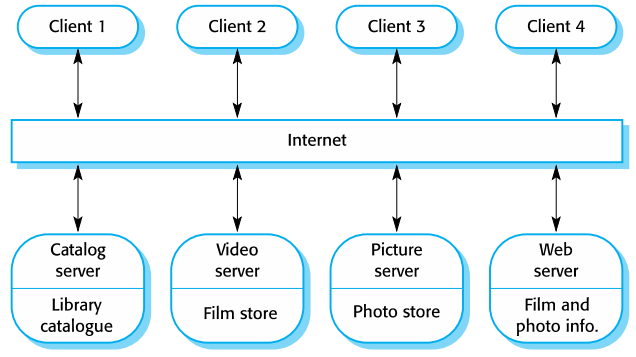
\includegraphics[width=0.55\linewidth]{images/client-server-architecture-film-library.PNG}
    \caption{Un'architettura client-server per una cineteca}
    \label{fig:client-server-architecture}
\end{figure}

Il catalogo deve essere in grado di gestire una varietà di query e fornire collegamenti al sistema informativo web che include dati sui film e sui videoclip, e a un sistema di e-commerce che supporta la vendita di fotografie, film e videoclip. Il programma client è semplicemente un'interfaccia utente integrata, costruita utilizzando un browser web, per accedere a questi servizi.

\subsection{Pipe and filter architecture}
Il pattern Pipe e Filter (Tabella \ref{tab:pipe-filter-pattern}) è un modello dell’organizzazione in fase di esecuzione di un sistema in cui trasformazioni funzionali processano i loro input e producono output. I dati fluiscono da un processo all’altro e vengono trasformati man mano che attraversano la sequenza. Ogni fase di elaborazione è implementata come una trasformazione.

Il nome “pipe e filtro” proviene dal sistema Unix originale, in cui era possibile collegare processi usando i “pipe” (condotti). Questi trasferivano un flusso di testo da un processo all’altro.

Varianti di questo pattern sono quando le trasformazioni sono sequenziali e i dati vengono processati in batch, questo modello architetturale a pipe e filtri diventa un modello sequenziale a batch, una struttura comune per sistemi di elaborazione dei dati.

\begin{table}[ht]
\centering
\rowcolors{2}{lightblue}{lightgray}
\begin{tabular}{|p{3cm}|p{11.5cm}|}
\hline
\rowcolor{headerblue}
\textbf{\textcolor{white}{Nome}} & \textbf{\textcolor{white}{Pipe e Filter}} \\\hline
Descrizione & L'elaborazione dei dati in un sistema è organizzata in modo che ogni componente di elaborazione (filtro) sia discreto e svolga un tipo di trasformazione dei dati. I dati fluiscono (come in un condotto) da un componente all'altro per l'elaborazione.\\\hline
Esempio & La Figura \ref{fig:pipe-filter-architecture} mostra un esempio di sistema pipe e filter utilizzato per l'elaborazione delle fatture.\\\hline
Quando utilizzarlo & Comunemente utilizzato in applicazioni di elaborazione dati (sia in batch che basate su transazioni) dove gli input vengono processati in fasi separate per generare output correlati.\\\hline
Vantaggi & Facile da comprendere e supporta il riutilizzo delle trasformazioni. Lo stile del flusso di lavoro si adatta alla struttura di molti processi aziendali. L'evoluzione attraverso l'aggiunta di trasformazioni è semplice. Può essere implementato sia come sistema sequenziale che concorrente.\\\hline
Svantaggi & Il formato per il trasferimento dei dati deve essere concordato tra le trasformazioni che comunicano. Ogni trasformazione deve analizzare il proprio input e convertire l'output nel formato concordato. Ciò aumenta il sovraccarico del sistema e può rendere impossibile il riutilizzo delle trasformazioni funzionali che utilizzano strutture dati incompatibili.
\\\hline
\end{tabular}
\caption{Il modello client-server}
\label{tab:pipe-filter-pattern}
\end{table}

Un esempio di questo tipo di architettura di sistema, usato in un'applicazione di elaborazione batch, è mostrato in Figura \ref{fig:pipe-filter-architecture}. Un'organizzazione ha emesso fatture per i clienti. Una volta alla settimana, i pagamenti effettuati vengono riconciliati con le fatture. Per le fatture che sono state pagate, viene emessa una ricevuta. Per quelle che non sono state pagate entro il termine di pagamento previsto, viene inviato un sollecito.

\begin{figure}[ht]
    \centering
    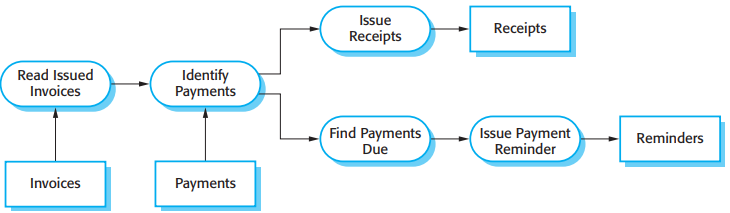
\includegraphics[width=0.75\linewidth]{images/pipe-filter-architecture.PNG}
    \caption{Un'architettura pipe and filter}
    \label{fig:pipe-filter-architecture}
\end{figure}

\section{Application architectures}
I sistemi applicativi sono progettati per soddisfare le esigenze di un'azienda o di un'organizzazione. Tutte le aziende hanno molte esigenze in comune: devono assumere personale, emettere fatture, mantenere contabilità e così via. Le aziende che operano nello stesso settore utilizzano applicazioni specifiche per quel settore. Di conseguenza, i sistemi applicativi utilizzati da queste aziende hanno molto in comune.

Queste somiglianze hanno portato allo sviluppo di architetture software che descrivono la struttura e l’organizzazione di particolari tipi di sistemi software. Le architetture applicative racchiudono le caratteristiche principali di una classe di sistemi. Questi sistemi hanno un'architettura e componenti standardizzati, che vengono configurati e adattati per creare una specifica applicazione aziendale.

Come progettista software, è possibile utilizzare modelli di architetture applicative in vari modi:
\begin{enumerate}
    \item Come punto di partenza per il processo di progettazione architetturale.
    \item Come lista di controllo per la progettazione.
    \item Come modo per organizzare il lavoro del team di sviluppo.
    \item Come mezzo per valutare i componenti per il riuso.
    \item Come vocabolario per parlare delle applicazioni.
\end{enumerate}
Esistono molti tipi di sistemi applicativi e, in alcuni casi, possono sembrare molto diversi. Tuttavia, applicazioni superficialmente dissimili possono avere molto in comune e quindi condividere un'architettura applicativa astratta. Illustrerò questo descrivendo le architetture di due tipi di applicazioni:
\begin{enumerate}
    \item \textit{Applicazioni di elaborazione delle transazioni:} Queste sono applicazioni incentrate sui database che elaborano richieste degli utenti per informazioni e aggiornano le informazioni in un database. Sono i tipi più comuni di sistemi aziendali interattivi. Sono organizzati in modo tale che le azioni degli utenti non possano interferire tra loro e venga mantenuta l'integrità del database. Questa classe di sistemi include sistemi bancari interattivi, sistemi di e-commerce, sistemi informativi e sistemi di prenotazione.
    \item \textit{Sistemi di elaborazione del linguaggio:} Sono sistemi in cui le intenzioni dell'utente sono espresse in un linguaggio formale, come un linguaggio di programmazione. Il sistema di elaborazione del linguaggio elabora questo linguaggio in un formato interno e poi interpreta questa rappresentazione interna. I sistemi di elaborazione del linguaggio più noti sono i compilatori, che traducono programmi di alto livello in codice macchina.
\end{enumerate}

\subsection{Sistemi di elaborazione delle transazioni}
I sistemi di elaborazione delle transazioni sono progettati per gestire le richieste degli utenti di informazioni da un database o le richieste per aggiornare un database.

Da una prospettiva dell'utente, una transazione è qualsiasi sequenza coerente di operazioni che soddisfa un obiettivo, come "trovare gli orari dei voli da Londra a Parigi".

I sistemi di elaborazione delle transazioni sono generalmente sistemi interattivi in cui gli utenti fanno richieste di servizio asincrone. La Figura \ref{fig:stracture-transaction-processing-app} illustra la struttura architetturale concettuale delle applicazioni di elaborazione delle transazioni. In primo luogo, un utente effettua una richiesta al sistema tramite un componente di elaborazione I/O. La richiesta viene elaborata da una logica specifica dell'applicazione. Viene quindi creata una transazione e passata a un gestore delle transazioni, solitamente integrato nel sistema di gestione del database. Dopo che il gestore delle transazioni ha verificato che la transazione è stata completata correttamente, segnala all'applicazione che l'elaborazione è terminata.

\begin{figure}[ht]
    \centering
    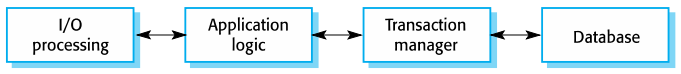
\includegraphics[width=0.70\linewidth]{images/stracture-transaction-processing-app.PNG}
    \caption{La struttura delle applicazioni di elaborazione delle transazioni}
    \label{fig:stracture-transaction-processing-app}
\end{figure}

I sistemi di elaborazione delle transazioni possono essere organizzati come un'architettura "pipe and filter", con componenti di sistema responsabili per l'input, l'elaborazione e l'output. Ad esempio, consideriamo un sistema bancario che consente ai clienti di consultare i loro conti e prelevare denaro da un bancomat. Il sistema è composto da due componenti software cooperanti: il software del bancomat e il software di elaborazione dei conti nel server di database della banca. I componenti di input e output sono implementati come software nel bancomat, mentre il componente di elaborazione fa parte del server di database della banca. La Figura \ref{fig:software-architecture-atm-system} mostra l'architettura di questo sistema, illustrando le funzioni dei componenti di input, processo e output.

\begin{figure}[ht]
    \centering
    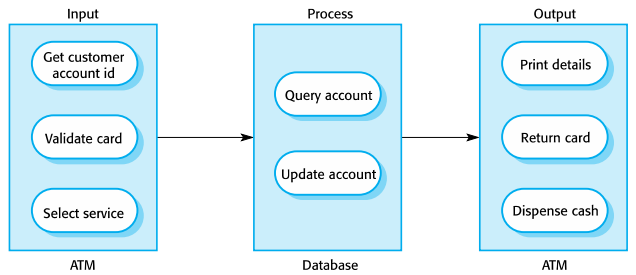
\includegraphics[width=0.60\linewidth]{images/software-architecture-atm-system.PNG}
    \caption{L'architettura software di un sistema ATM}
    \label{fig:software-architecture-atm-system}
\end{figure}

\subsection{Sistemi informativi}
Un sistema informativo consente un accesso controllato a una grande base di informazioni. I sistemi informativi sono quasi sempre sistemi basati su web, dove l'interfaccia utente è implementata in un browser web.

La Figura \ref{fig:layered-information-system-architecture} presenta un modello molto generale di un sistema informativo. Il sistema è modellato utilizzando un approccio a livelli in cui il livello superiore supporta l'interfaccia utente e il livello inferiore è il database del sistema. Il livello di comunicazione con l'utente gestisce tutti gli input e output dall'interfaccia utente, mentre il livello di recupero delle informazioni include la logica specifica dell'applicazione per accedere e aggiornare il database.

\begin{figure}[ht]
    \centering
    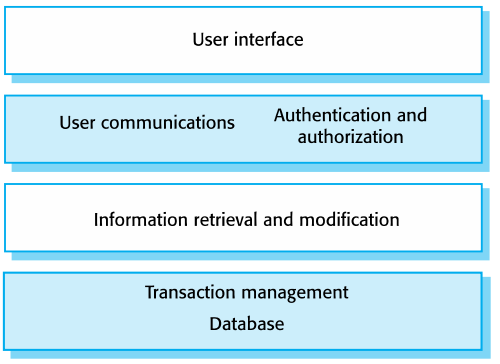
\includegraphics[width=0.42\linewidth]{images/layered-information-system-architecture.PNG}
    \caption{Architettura del sistema informativo stratificato}
    \label{fig:layered-information-system-architecture}
\end{figure}

Come esempio di istanza di questo modello a livelli, la Figura \ref{fig:architecture-mentcare-system} mostra l'architettura del sistema Mentcare:

\begin{figure}[ht]
    \centering
    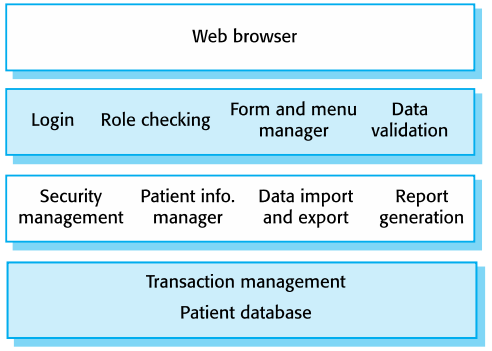
\includegraphics[width=0.42\linewidth]{images/architecture-mentcare-system.PNG}
    \caption{L'architettura del sistema Mentcare}
    \label{fig:architecture-mentcare-system}
\end{figure}

\begin{enumerate}
    \item Il livello superiore è un'interfaccia utente basata su browser.
    \item Il secondo livello fornisce le funzionalità dell'interfaccia utente che sono erogate tramite il browser web.
    \item Il terzo livello implementa le funzionalità del sistema e fornisce componenti che implementano la sicurezza del sistema, la creazione e l'aggiornamento delle informazioni sui pazienti, l'importazione e l'esportazione di dati dei pazienti da altri database e generatori di report che creano report di gestione.
    \item Infine, il livello inferiore, costruito utilizzando un sistema di gestione di database commerciale, fornisce la gestione delle transazioni e la memorizzazione persistente dei dati.
\end{enumerate}
I sistemi di gestione delle informazioni e delle risorse sono talvolta anche sistemi di elaborazione delle transazioni. Ad esempio, i sistemi di e-commerce sono sistemi di gestione delle risorse basati su Internet che accettano ordini elettronici per beni o servizi e quindi organizzano la consegna di questi beni o servizi al cliente. In un sistema di e-commerce, il livello specifico dell'applicazione include funzionalità aggiuntive che supportano un "carrello" in cui gli utenti possono inserire diversi articoli in transazioni separate e poi pagarli tutti insieme in un'unica transazione.

Questi sistemi sono spesso implementati come sistemi distribuiti con un'architettura client-server multi-tier:
\begin{enumerate}
    \item Il server web è responsabile di tutte le comunicazioni con l'utente, con l'interfaccia utente implementata utilizzando un browser web;
    \item Il server applicativo è responsabile dell'implementazione della logica specifica dell'applicazione e delle richieste di memorizzazione e recupero delle informazioni;
    \item Il server di database sposta le informazioni da e verso il database e gestisce la gestione delle transazioni.
\end{enumerate}

\subsection{Sistemi di elaborazione del linguaggio}
I sistemi di elaborazione del linguaggio traducono un linguaggio in una rappresentazione alternativa di quel linguaggio.

Una possibile architettura per un sistema di elaborazione del linguaggio per un linguaggio di programmazione è illustrata nella Figura \ref{fig:architecture-language-processing-system}. Le istruzioni del linguaggio sorgente definiscono il programma da eseguire, e un traduttore le converte in istruzioni per una macchina astratta. Queste istruzioni vengono quindi interpretate da un altro componente che le preleva per eseguirle e le esegue utilizzando (se necessario) i dati dall'ambiente. L'output del processo è il risultato dell'interpretazione delle istruzioni sui dati di input.

\begin{figure}[ht]
    \centering
    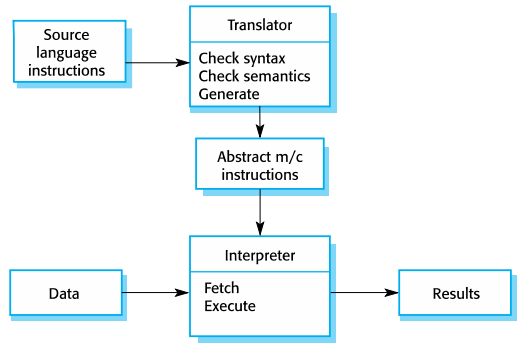
\includegraphics[width=0.52\linewidth]{images/architecture-language-processing-system.PNG}
    \caption{L'architettura di un sistema di elaborazione del linguaggio}
    \label{fig:architecture-language-processing-system}
\end{figure}

I compilatori dei linguaggi di programmazione che fanno parte di un ambiente di programmazione più generale hanno un'architettura generica (Figura \ref{fig:repository-architecture-language-processing-system}) che include i seguenti componenti:
\begin{enumerate}
    \item Un analizzatore lessicale, che prende i token di input del linguaggio e li converte in una forma interna.
    \item Una tabella dei simboli, che contiene informazioni sui nomi delle entità (variabili, nomi di classi, nomi di oggetti, ecc.) utilizzati nel testo che viene tradotto.
    \item Un analizzatore sintattico, che controlla la sintassi del linguaggio in fase di traduzione.
    \item Un albero sintattico, che è una struttura interna che rappresenta il programma in fase di compilazione.
    \item Un analizzatore semantico, che utilizza le informazioni dall'albero sintattico e dalla tabella dei simboli per verificare la correttezza semantica del testo di input del linguaggio.
    \item Un generatore di codice, che "percorre" l'albero sintattico e genera codice per una macchina astratta.
\end{enumerate}

\begin{figure}[ht]
    \centering
    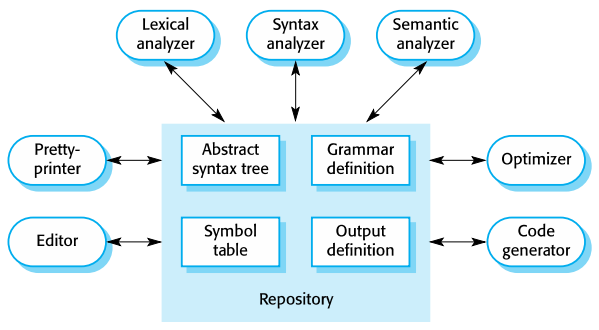
\includegraphics[width=0.52\linewidth]{images/repository-architecture-language-processing-system.PNG}
    \caption{Un'architettura di repository per un sistema di elaborazione del linguaggio}
    \label{fig:repository-architecture-language-processing-system}
\end{figure}

La Figura \ref{fig:pipe-filter-compiler-architecture} illustra come un sistema di elaborazione del linguaggio possa essere parte di un insieme integrato di strumenti di supporto alla programmazione. In questo esempio, la tabella dei simboli e l'albero sintattico agiscono come un repository centrale di informazioni. 

\begin{figure}[ht]
    \centering
    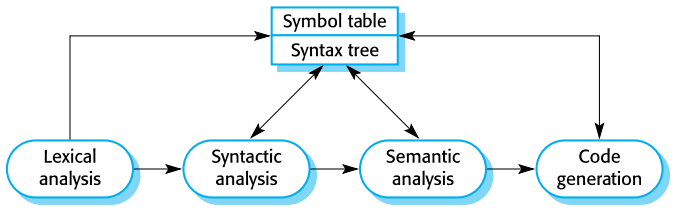
\includegraphics[width=0.55\linewidth]{images/pipe-filter-compiler-architecture.PNG}
    \caption{Un'architettura di repository per un sistema di elaborazione del linguaggio}
    \label{fig:pipe-filter-compiler-architecture}
\end{figure}

I compilatori possono essere implementati utilizzando un modello composito di repository e pipe and filter. In un'architettura del compilatore, la tabella dei simboli è un repository per i dati condivisi. Le fasi di analisi lessicale, sintattica e semantica sono organizzate in sequenza, come mostrato nella Figura \ref{fig:pipe-filter-compiler-architecture}, e comunicano attraverso la tabella dei simboli condivisa.

\section{Punti chiave}
\begin{center}
\begin{minipage}{\textwidth}
\colorbox{lightgray}{
\parbox{\linewidth}{
\begin{itemize}
    \item Un'architettura software è una descrizione di come è organizzato un sistema software.
    \item Le decisioni di progettazione architetturale includono la scelta del tipo di applicazione, la distribuzione del sistema e gli stili architetturali da utilizzare.
    \item Le architetture possono essere documentate da diverse prospettive o viste, come una vista concettuale, una vista logica, una vista di processo e una vista di sviluppo.
    \item I pattern architetturali sono un mezzo per riutilizzare la conoscenza delle architetture di sistema generiche. Descrivono l'architettura, spiegano quando può essere utilizzata e ne descrivono vantaggi e svantaggi.
    \item I modelli delle architetture dei sistemi applicativi ci aiutano a comprendere e confrontare le applicazioni, a convalidare i progetti dei sistemi applicativi e a valutare i componenti su larga scala per il riutilizzo.
    \item I sistemi di elaborazione delle transazioni sono sistemi interattivi che consentono a più utenti di accedere e modificare in remoto le informazioni in un database.
    \item I sistemi di elaborazione del linguaggio vengono utilizzati per tradurre testi da un linguaggio a un altro e per eseguire le istruzioni specificate nel linguaggio di input. Includono un traduttore e una macchina astratta che esegue il linguaggio generato.
\end{itemize}
}}
\end{minipage}
\end{center}